\section{Laser Induced Graphene}


\subsection{Direct Laser Scribing Carbonization}
%Various Types. LIG Porous, LIG Fibers, Lift off LIG, Chess like LIG. Sample preparation.

In the present work laser induced graphene materials were produced via pyrolysis process in ambient conditions by the commercially available laser cutter/engraver system VLS 2.30 from Universal Laser System. The laser system is equipped with a 30W CO$_2$ laser source at 10.6 $\mu$m wavelength, operating with a pulse repetition frequency f$_{rep}$ = 5 kHz. Raster laser scribing is done at speeds varying from 100 to 830  mm/s. The lens system used is the HPDFO (High Power Density Focusing Optics) which provides a focused beam spot size of 30 $\mu$m. 

Laser irradiation of polyimide (PI) films, adhesive tapes as well as of polyether ether ketone (PEEK) films enabled direct induction of the graphene formation via a carbonization process as schematically shown in Figure \ref{fig:LIG_formation}. As a result of laser processing the integrity of the pyrolized film is not completely compromised since a residual part of the initial polymer remains under the LIG allowing it to act as mechanical support.

\begin{figure}[H]
\centering
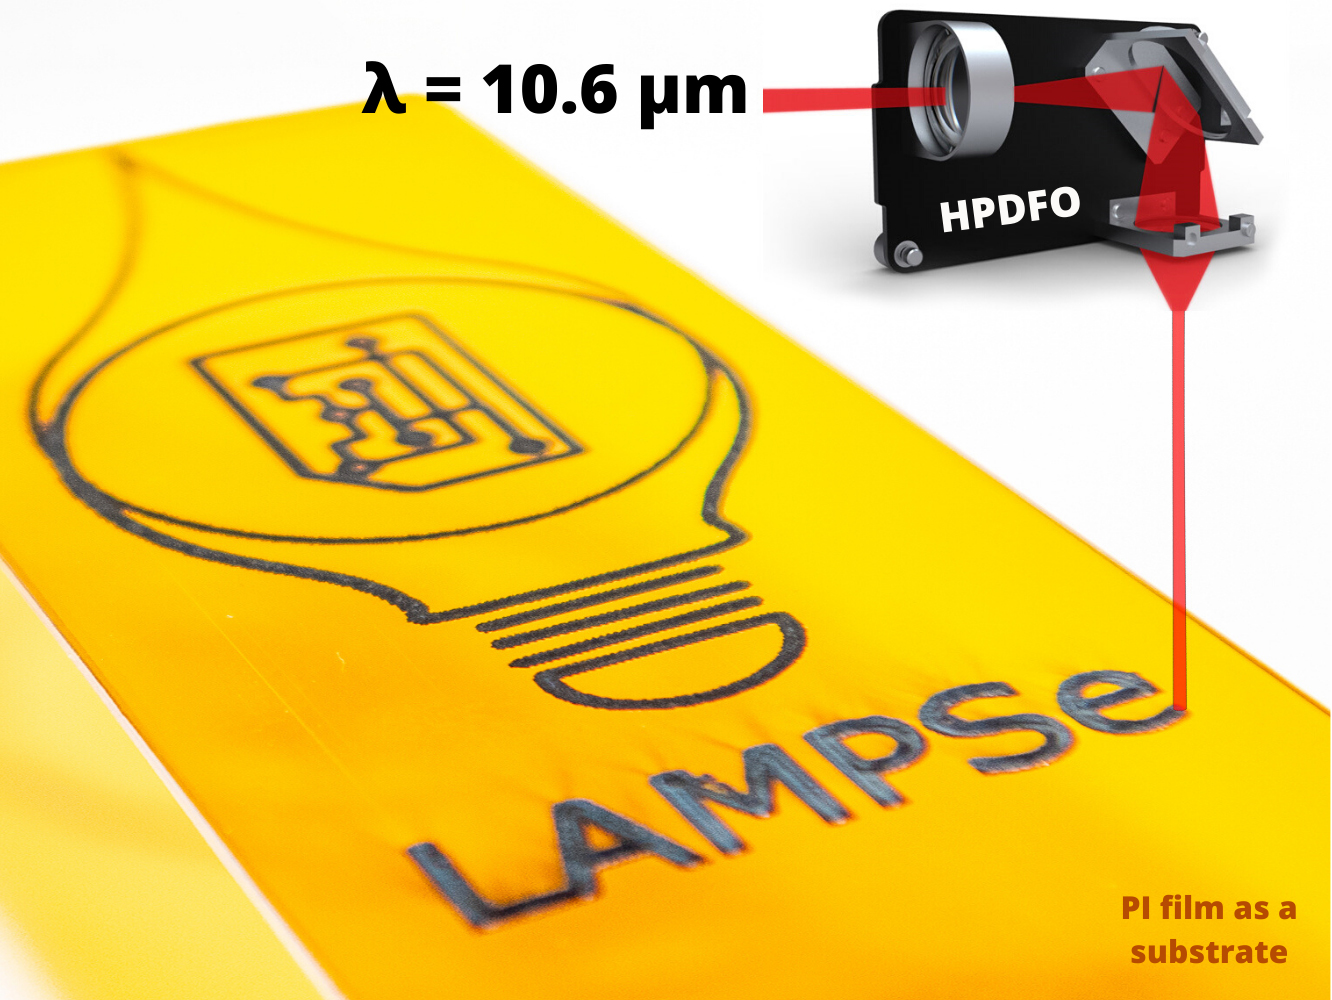
\includegraphics[width=0.5\textwidth]{Figures/ExperimentalSetup/LIG-LAMPSE.jpg}
\medskip
\caption{LIG formation by laser beam treatment}
\label{fig:LIG_formation}
\end{figure}

Depending on the laser settings such as laser power, speed of scanning, plane height Z-position as compared to the focal point, raster resolution  and amount of scanning lines per scribed area (Image Density) the laser fluence $H$, that is amount of optical energy delivered per surface area $J/m^2$, can be varied. Fluence values in turn affect the final photothermal processes leading to the polymer pyrolysis and LIG formation. Tuning of fluence controls the structure (i.e. amount of crystalline/amorphous carbon) and morphology of the produced LIG.

Earlier \cite{duy_laser-induced_2018} it was found that by utilizing the interplay of the varied laser settings two main morphologies of LIG can be obtained on PI Kapton$^{TM}$ films. In order to tune the aforementioned parameters for obtaining laser fluence values $H$ leading to a particular microstructure of the obtained graphene material, a separate study was conducted by Hana Hampel in her master thesis \cite{hana}. As a result of the described work, it was possible to establish a one-to-one correspondence between the laser settings (power, scanning speed, raster resolution, image density and defocus distance) and $H$. In the Figure \ref{fig:LIG-map} obtained by Hana Hampel \cite{hana}, it is shown how the appearance of the carbon material changes upon the laser settings. For each single Power\%-Speed\% configurations the laser fluence $H$ was calculated and the results were layered on top of the mapping with a colour code as shown on the right side. The H-trend corresponded very well to the obtained morphology. 

\begin{figure}[H]
\centering
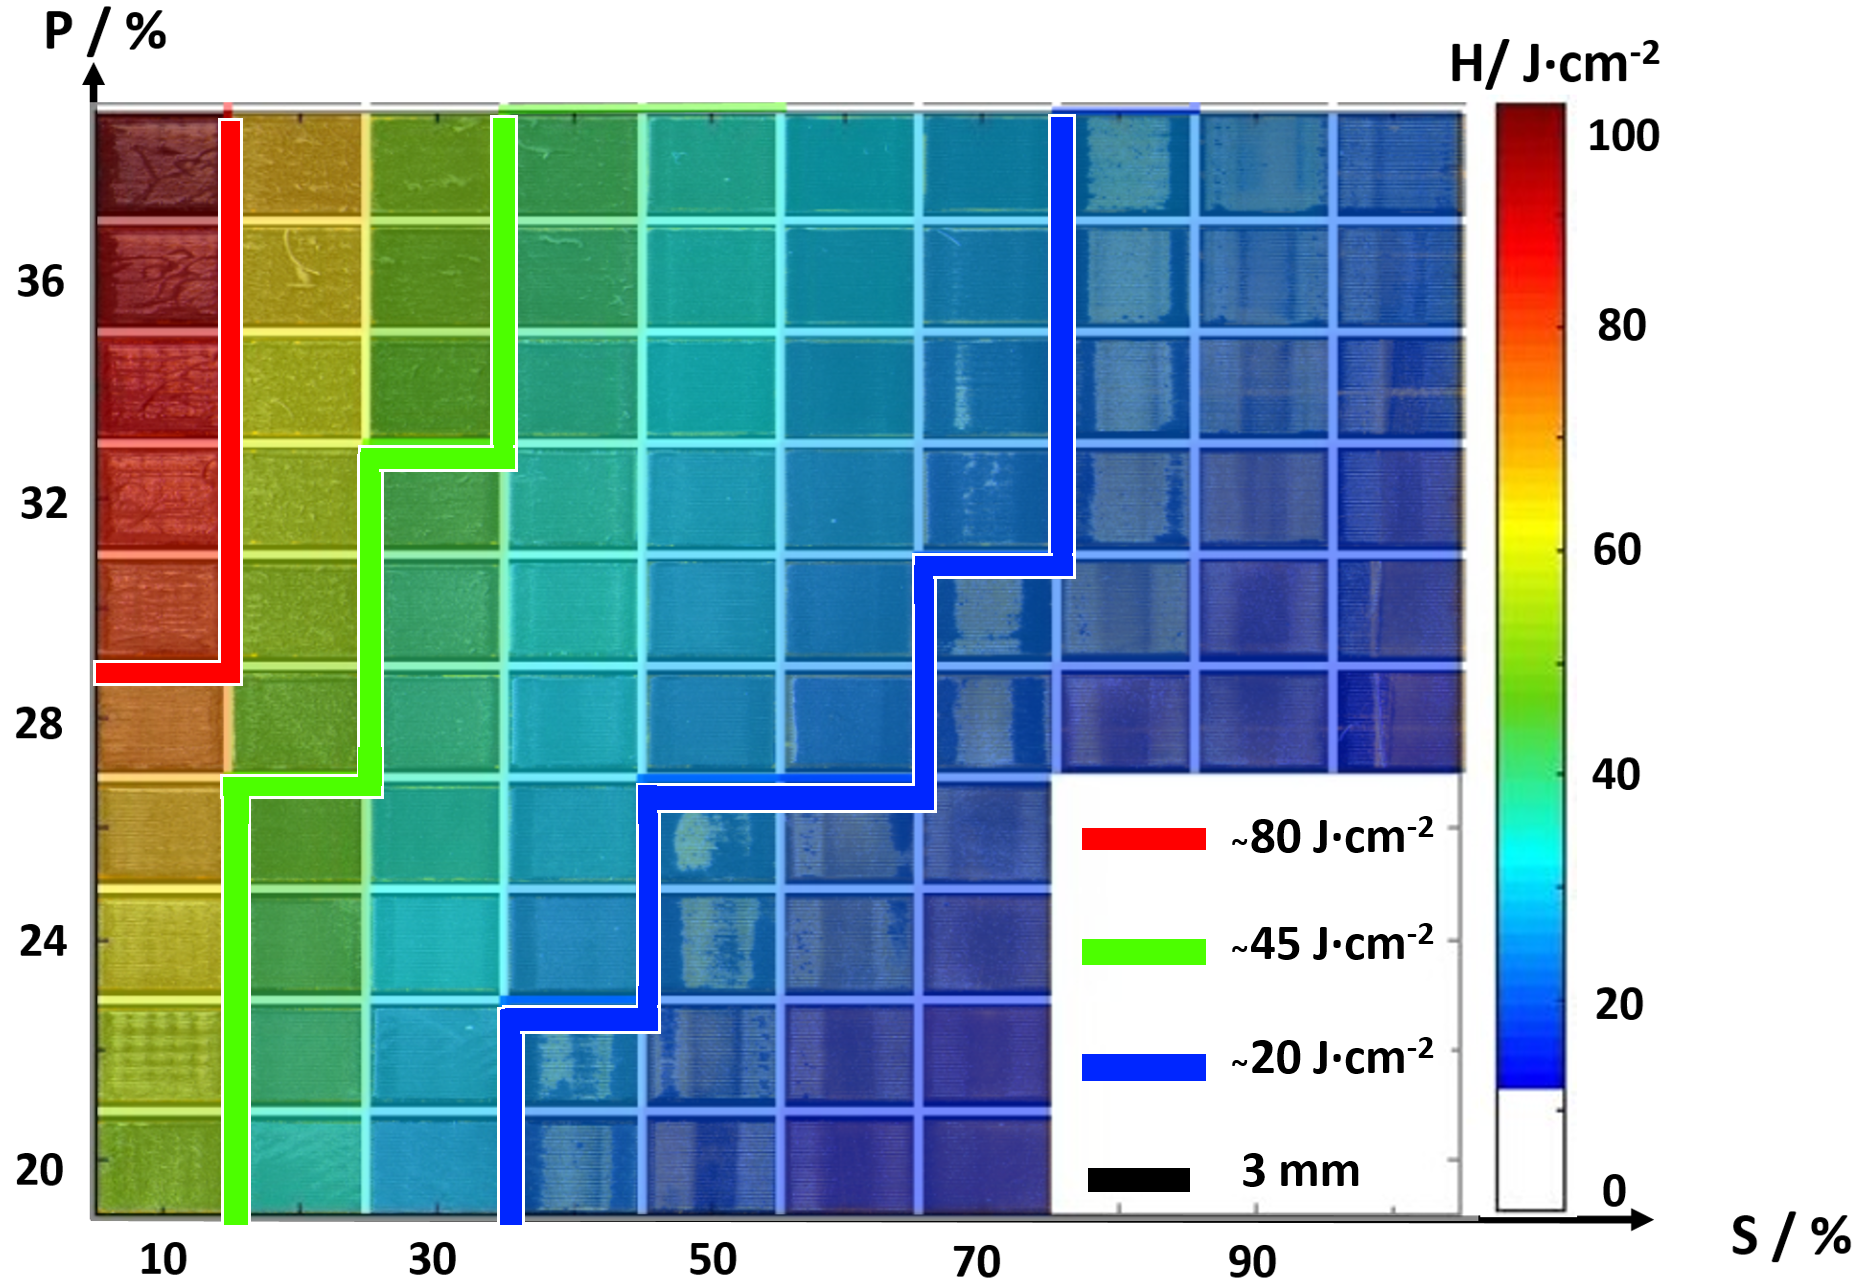
\includegraphics[width=1\textwidth]{Figures/ExperimentalSetup/H_mapping_results.PNG}
\medskip
\caption{Map of LIG obtained on Kapton$^{TM}$ 50 $\mu$m film showing variations upon the laser power within the range between 20$\%$ - 40$\%$ and speed between 10$\%$ - 100$\%$. For laser fluence values $H < (20 \pm 2) J \times cm^{-2}$ (blue area) no homogeneous LIG formation was found. Flat-LIG was obtained in the range $(20 \pm 2) < H < (45 \pm 5) J \times cm^{-2}$ and LIG-fibres for $(45 \pm 5) < H < (80 \pm 8) J \times cm^{-2}$ (green area). The red area, referred to the destroyed polymer sheet, lied in the range $H > (80 \pm 8) J \ cm^{-2}$ \cite{hana}}
\label{fig:LIG-map}
\end{figure}

In this work two sets of settings were used for LIGs preparations. Different LIG types were achieved by varying laser power and Z-distance value, which is the offset position of the substrate relatively to the focal point of the laser varied. The other scribing settings were kept constant as follows: the point per inch (PPI) value was always set to 500, the image density (ID) was set to 5 a.u. (corresponding to a 280 $\mu$m spacing between consecutive lines) and the rastering speed was set to 10$\%$ which corresponds to 100 $\pm$ 10 mm/s. 

Firstly a highly porous conductive carbon material, in our work denoted as LIGP, which appears in the form of ultrathin black flakes stacked on the surface of the polymeric substrate, was obtained at the laser power value set to 11$\%$. According to the fluence calculations of Hana Hampel \cite{hana} that corresponds to $H$ being approx. $\approx25 J/cm^2$. Another LIG type, called LIGF in this thesis, was obtained at power of 20$\%$, which corresponds to $H = \approx50 J/cm^2$. This yielded formation of structures having porous-like material in the bottom layers whereas the top layers consist of fibers. The images of the LIGs obtained with scanning electron microscopy (SEM) can be found in the Results Section at Figure \ref{fig:LIGs-SEMs}.

 //A special type of LIGP, called LIGP LIFT OFF is obtained with high speed settings. This LIG type can be easily peeled off from the precursor substrate and its processing has been optimized for preparing flexible composites. //


As LIG precursors we used two types of polyimide material which we distinguish as \textbf{Kapton$^{TM}$ Film}, a bare polyimide foil, and \textbf{Kapton$^{TM}$ Tape}, which is a polyimide foil with a polyacrylic adhesive layer on one side. Both materials are produced by DuPont. The PEEK film used is produced by RS PRO Company. Before laser scribing the non-adhesive foils were put onto a aluminum 1 mm thick plate and fixed via duct tape. The adhesive precursors were fixed onto 1 mm thick glass slabs. The top surface of the samples was rinsed with isopropanol. 

Table \ref{tab:ligtypes} sums up the LIG types which were prepared.  

\begin{table}[H]
\centering
    \caption{Polymeric LIG-sources and LIG Types used in this work.}
    \label{tab:ligtypes} 
\medskip
\medskip
\begin{tabular}{c| c| c| c| c } 

   LIG-Source Material & LIG Notation & Power [\%] & Speed [\%] & Z-distance [mm] \\[13px]
   \hline
     Kapton$^{TM}$ Film 50 $\mu$m  & LIGP   & 11 & 10  & 2 \\[13px]
                                  & LIGF   & 20 & 10 & 1.7 \\[13px]
   \hline
                                  & LIGP   & 11 & 10 & 2 \\[13px]
    Kapton$^{TM}$ Tape 50 $\mu$m               & LIGP LIFT OFF  & 11 & 10 & 2 \\[13px]
                                  & LIGF   & 20 & 10 & 1.7 \\[13px]
   \hline
     PEEK Film 100 $\mu$m           & LIGP   & 11 & 10 & 2 \\[13px]

\end{tabular}
\end{table}


Flexibility of the lasered pattern design enabled us to prepare conductive devices of various flat shapes which will be further described in the respective sections.

\subsection{Conductive Elastic Biocomposites Based on LIG}
\label{composites_preparation}

\medskip
\textbf{LIG-PDMS Composite}

Polydimethylsiloxane (PDMS, Sylgard 184, Dow Corning, Midland, MI, USA) was used as an elastomeric matrix material for LIG  composites. After mixing prepolymer base and curing agent (8/1 w/w ratio) the mixture was degassed in vacuum for 10 minutes before to pour it onto the desired substrates for LIG encapsulation and cured (see details in following). In this thesis this PDMS material will be denoted as PDMS-8:1. The ratio used here was chosen as it allowed an easier peeling off process of LIG from the PI precursor.  

The Kapton$^{}$ film or Kapton$^{}$ adhesive tape was put on top of a 70 x 25 mm glass slab and the desired LIG pattern was laser scribed. For the case of Kapton$^{}$ film it was fixed to the glass slab by as double side adhesive tape XXXX. One part of freshly prepared PDMS mixture was spin coated on top of LIG pattern. The spin coating settings of the used XXXX device were set to the following parameters:

\begin{itemize}
\item spin speed: 600 $rpm$
\item spin acceleration: 100 $rpm/s$
\item spining time: 60 $s$
\end{itemize}

Spin-coated samples were cured at 80 $\degree$C for 20 minutes, after which a second layer of PDMS was spin coated with the same parameters on the top of the first one. Afterwards the samples were finally cured at  80 $\degree$C for 3 hours. Subsequently the specimen were submerged into ethyl acetate solvent (Merck) for 5 - 10 minutes. This step enabled smooth peeling of the thin composite LIG-PDMS films from the original polyimide substrates. The workflow of the composite production process is illustrated in the Figure \ref{fig:PDMS_LIG_production}.

\begin{figure}[H]
\centering
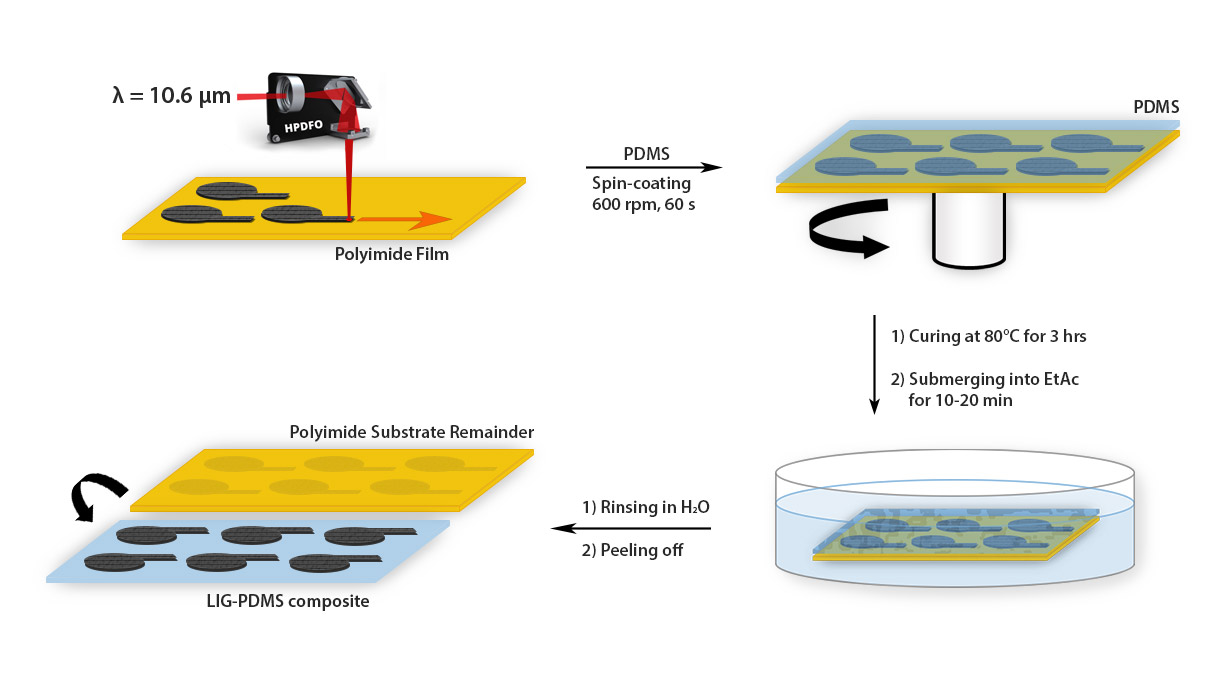
\includegraphics[width=1\textwidth]{Figures/ExperimentalSetup/LIG_PDMS_Production.jpg}
\medskip
\caption{Preparation of LIG-PDMS Composite}
\label{fig:PDMS_LIG_production}
\end{figure}

\medskip
\textbf{LIG-MPU Composite}

Another type of stretchable LIG composite was prepared by transferring the LIG patterns onto a commercially available medical polyurethane film (MPU) (Fixomull$^{TM}$ transparent, BSN Medical). It constitutes an ultrathin transparent and waterproof viscoelasitc film coated with a skin-friendly polyacrylate adhesive.

The technical data for MPU film particularly used in this work is presented in Table \ref{tab:MPU_tech}

\begin{table}[H]
\centering
    \caption[Caption for LOF]{Medical grade Polyurethane Film \cite{Fixomull_tech_data}}
    
    \label{tab:MPU_tech} 
\medskip
\medskip
\begin{tabular}{ l | l } 

Property & Typical Value  \\[15px]
\hline

Thickness [$\mu m$] & 28 \\[15px]
Weight [$g/m^2$] & 30 \\[15px]
Moisture vapor transmission rate upright [$g/m^2$ per 24hrs at 37$\degree C$] & 1400\\[15px]
Tensile Strength [MPA] & 0.1\\[15px]
Elongation at break, MD ($\%$) & 650\\[15px]

\end{tabular}
\\[15px]

\end{table}


The film has two protection liners: the polyacrylate glue side (bottom) is covered with a glassine paper and the top polyurethane side is covered with a plastic support/release liner. Before transfer the glue side was masked to match the LIG pattern. The mask was prepared via the laser cutter by cutting out the respective pattern only in the glassine paper on the adhesive side of the film. The laser cutter settings were as follows: Power = 2.2\%, Speed = 9\%, PPI = 500, ID = 5, z-defocus of 1 mm). After this procedure the respective parts of the liner were removed to match the shape of the LIG device. The MPU film was put onto the scribed LIG pattern and a pressure was applied with the help of a cotton tip in order to transfer the LIG material onto the MPU film as it is schematically shown in stages i-iv in Figure \ref{fig:MPU_LIG_production}. 

\begin{figure}[H]
\centering
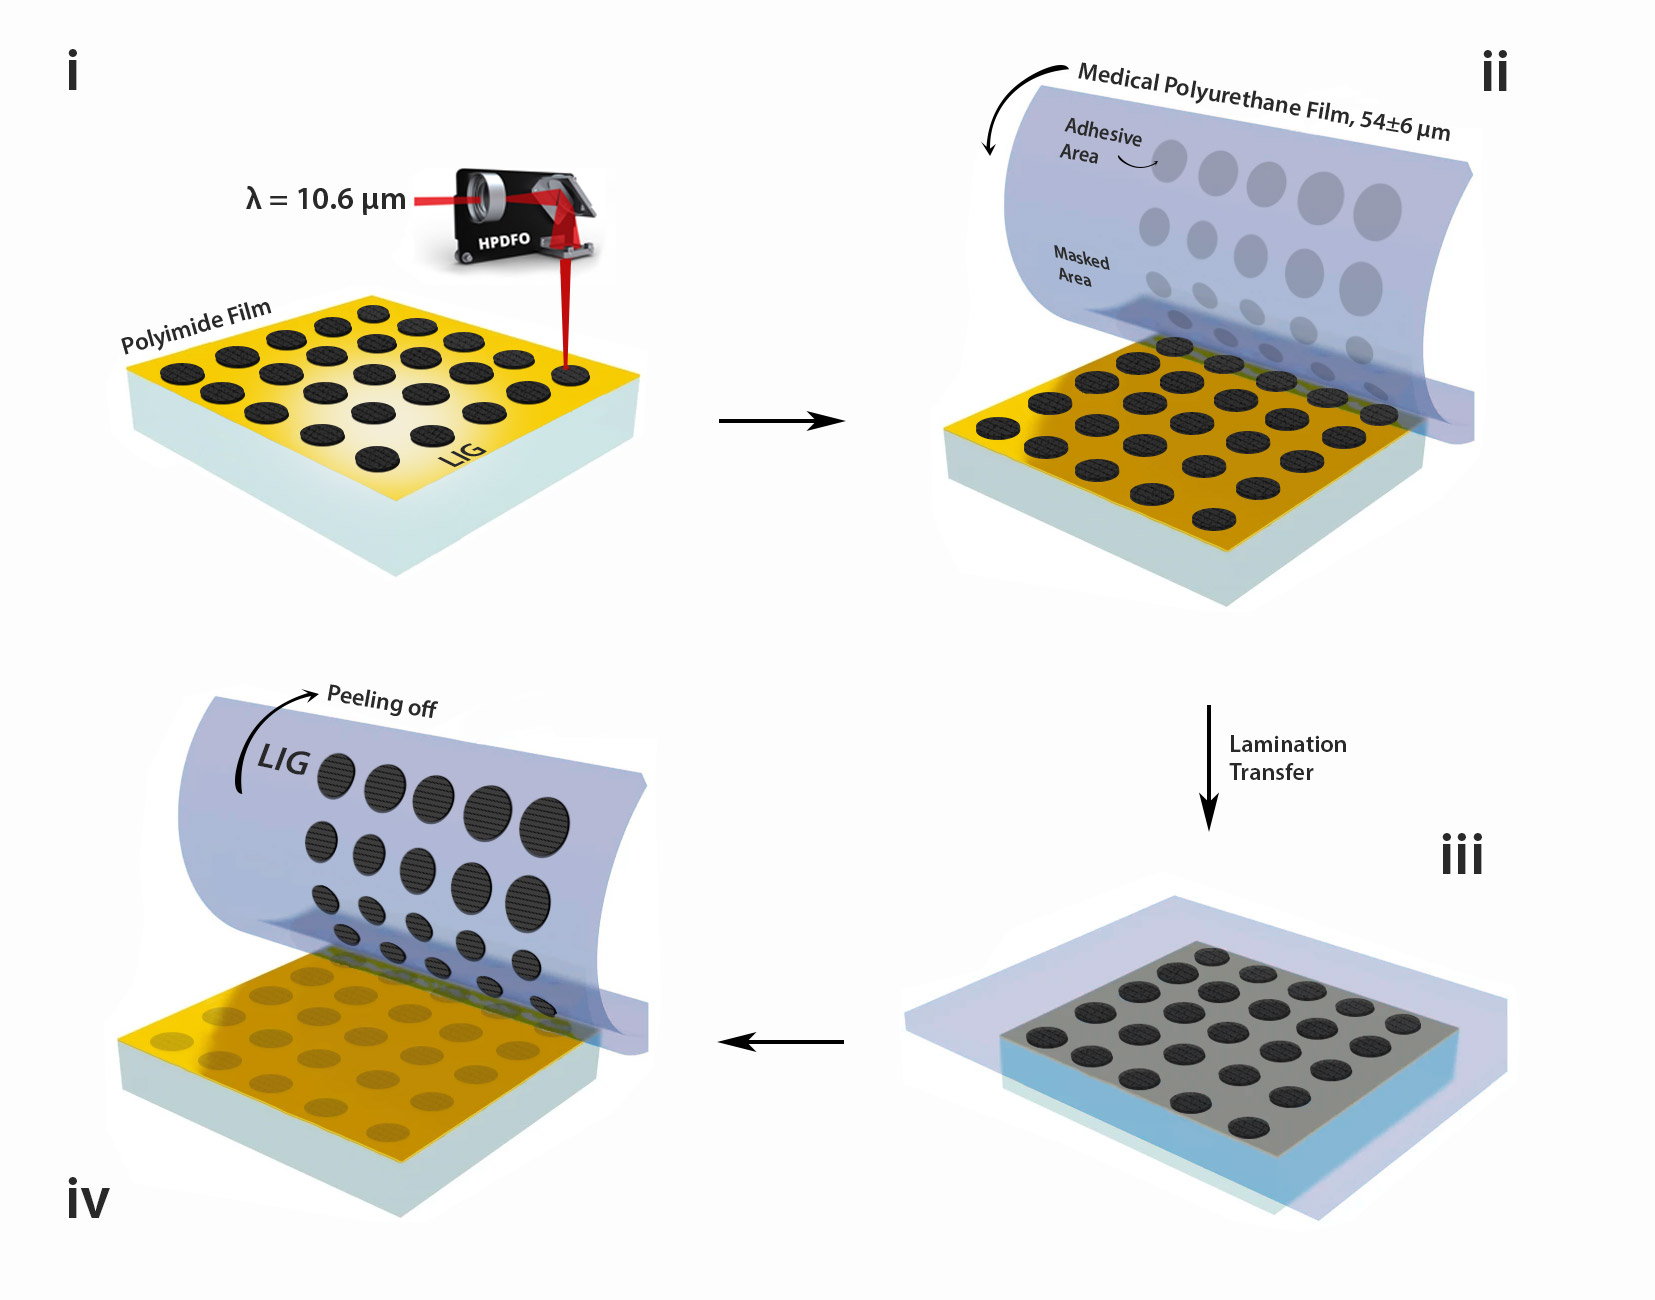
\includegraphics[width=1\textwidth]{Figures/ExperimentalSetup/LIG_Fixomull_Production.jpg}
\medskip
\caption{Preparation of LIG-MPU Composite. (i) Laser scribing on polyimide film for LIG creation; (ii-iv) schematics of LIG lamination transfer onto MPU
}
\label{fig:MPU_LIG_production}
\end{figure}


\section{LIG Materials Characterization}


\subsection{Imaging Techniques}

The optical imaging of LIG materials and the LIG based composites was performed with a Leica Wild M3B ligth microscope. SEM images were obtained with a JEOL JSM-6490LV Scanning Electrode Microscope, operating at 5 kV to 20 kV acceleration voltage.

\subsection{Mass Density Characterization of LIGs}

Further investigations required an estimation of the LIG mass per substrate area. Thus the mass of LIG per surface area was evaluated for PI, PEEK, PDMS and MPU substrates. LIG patterns (10$\:$mm in diameter) were laser scribed in raster mode with the respective LIGP and LIGF settings, see section X.X. Afterwards circles were cut out with laser operating at X, Y, Z in vector mode.  At first each circle was accurately weighed on the ???XXXX microbalance. To measure the mass of LIG scribed on the PI and on the PEEK films the LIG was scraped off from the surface with the aid of a scalpel blade and the mass of the resting round shaped substrate was measured again. To measure the mass of the LIG material transferred to the MPU adhesive band, the mass of the original LIG-PI circles was measured, after which the LIG was transferred by lamination technique to the PU and the rest mass of the LIG-PI samples was measured again. The difference between the first and the second results was taken as the LIG mass value. The balancing error was 0.0001 g. For the Kapton Film and Kapton Tape the mass densities of respective LIG types were assumed to be equal. 

For each type of substrate the procedure was repeated three times and the mass per surface was calculated as the averaged mean value of these three results. For the LIG+PDMS composites it was assumed that all LIG material is transferred from the PI foil, which was in a satisfying agreement with the light microscopy investigation of the resting PI film.

The summary of the obtained values can be found in Table \ref{tab:LIG_mass} in the Results Section \ref{chapter:Results and discussion}.


\subsection{Thickness Measurements}

The thickness measurement of Kapton$^{TM}$ film and tape was performed with a stylus profilometer AlphaStep D-500 from KLA-Tencor operating with a scan length of 5mm, speed set to 0.1 mm/s and loading stylus force set to 1 mg. For each sample, one for Kapton$^{TM}$ film and another one for Kapton$^{TM}$ tape, at least five measurements per sample were done and the result was taken as a mean average value.
 
The profilometer set up did not allow to proceed with the thickness measurements for softer materials, such as PDMS. Therefore the evaluation were done by the means of a light microscope by comparing the thickness of thin slices of the investigated soft samples against the slices with the known thickness. The estimations were done in five different points and the final result was taken as a range of the obtained values. In order to minimize the uncertainties, which are associated with the described technique, it was made sure that the cross-sections were sliced normal to the film plane and that the slices in turn were then placed normal to the focal plane of the light microscope.

\subsection{Electromechanical Characterization of Composites}

\medskip
\textbf{Electromechanical Stretching Setup}
The change in electrical resistance of LIGs supported by various substrates to the imposed strain was measured via a custom setup built by A. Dallinger from LAMPSe group (shown in Figure \ref{fig:stretcher}). The composite sample is mounted between two holders, with one of them fixed to a stage moved by a stepper motor, and the other fixed to a load cell Futek LRF400 with an Amplifier Futek IAA100 to measure the stress imposed on the mounted sample.  During the electromechanical tensile tests the load values are read out as an analogue signal via an Arduino microcontroller. The sample holders provide at the same time an electrical contact to the sample through copper plate electrodes.  The resistance across the stretched sample is measured via a Keithley 2601B Source Meter sourcing 10 mA. Controlled strain is imposed on samples by means of a NEMA 17 stepper motor controlled by an Arduino microcontroller. A custom C\texttt{\#} software was used to communicate with Arduino and to record the measurements. 

\begin{figure}[H]
\centering
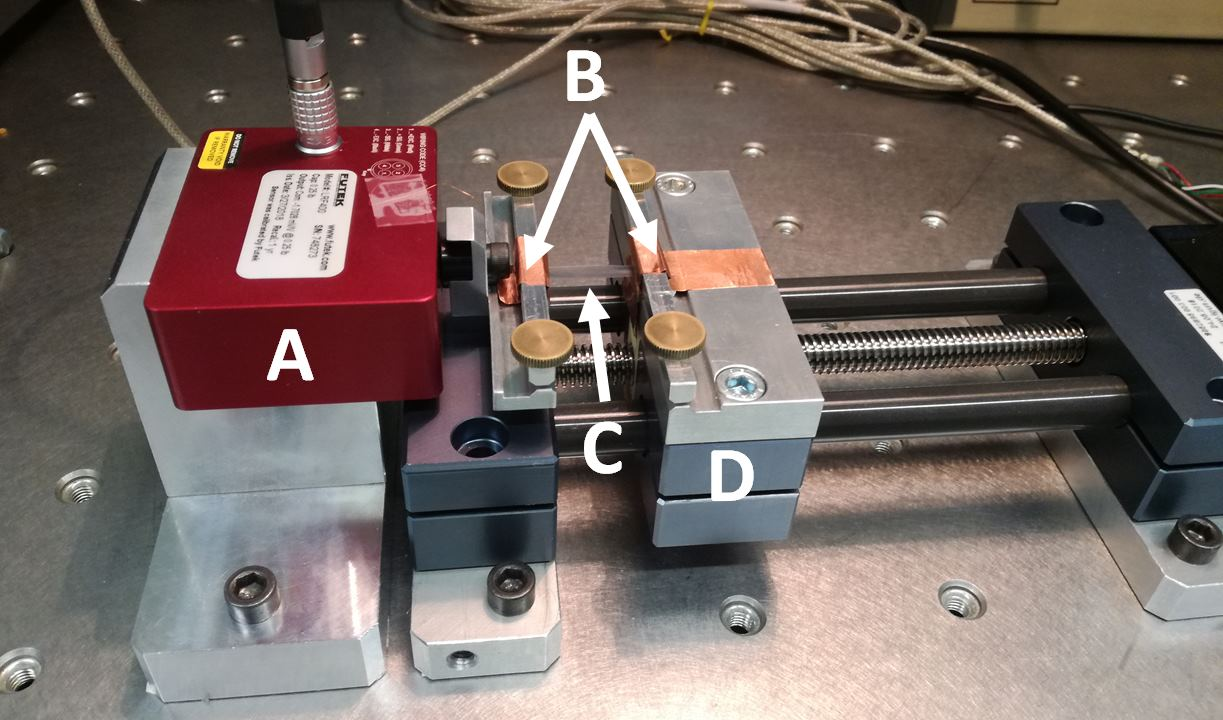
\includegraphics[width=1\textwidth]{Figures/ExperimentalSetup/Stretcher.jpg}
\medskip
\caption{Electromechanical test setup consisting of load cell (A), electrical contacts (B), sample (C) and movable stage (D) \cite{Dallinger}
}
\label{fig:stretcher}
\end{figure}

\medskip
\textbf{Humid Chamber Setup}

One of the goals of this thesis was to investigate the electromechanical behaviour of the LIG composites in ambient conditions with varying relative humidity (RH$\%$). This aim required building up a humid chamber around the Stretcher so that the RH of the ambient air around the electromechanically tested specimen could be dynamically regulated and controlled.

The described setup is shown in Figure \ref{fig:humid_setup}. It consisted of a polystyrene chamber \textbf{A} (built by the LAMPSE bachelor student David Grafinger), a commercially available humidity source (AGPTEK 400mL/H Mini Mist Maker) \textbf{B}, an DHT22 humidity sensor \textbf{C}, controlled by an Arduino Uno$^{TM}$ board and a set of fans \textbf{D}. The moisture level in the chamber could be regulated by the size of the openings for the fans. RH$\%$ was controlled by the readings from the DHT22 sensor sent over to a PC interface by the pre-programmed Arduino setup. 

\medskip
\textbf{Tested Specimen}

Test samples were prepared as 40mm x 5mm stripes of LIG supported by various substrates as according to the Table \ref{tab:LIG_stripes_electromechanical_tests}. Since the laser rastering  causes the LIG patterns to have anisotropy in their microstructure, for each combination of LIG/Substrate two types of stripes were prepared: with the laser scribing either parallel to the main axis of the stripe (LIG$\parallel$) or normal to it (LIG$\bot$). 

For the mounting setup 5 mm wide areas on the tips of the samples were left clear of LIG so the real part imposed to the strain had a length at around (30$\pm$2)mm as shown in Figure \ref{fig:stretching_specimen}. 

\begin{figure}[H]
\centering
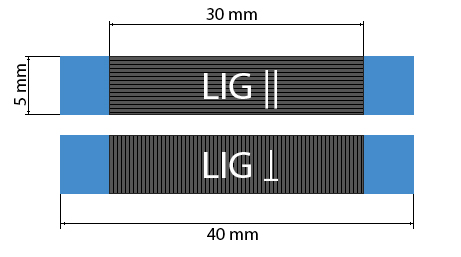
\includegraphics[width=0.5\textwidth]{Figures/ExperimentalSetup/Stretching-Specimen.jpg}
\medskip
\caption{Schematics of samples for electromechanical measurements}
\label{fig:stretching_specimen}
\end{figure}

\begin{table}[H]
\centering
    \caption{List of Samples for Electromechanical Tests}
    \label{tab:LIG_stripes_electromechanical_tests} 
\medskip
\medskip
\begin{tabular}{ l | l | l  } 

Sample Type $\#$& LIG Type\footnotemark[1] & Substrate \\[15px]
\hline
1 & LIGP$\parallel$ / LIGP$\bot$    & PDMS-8:1 \\[13px]
2 & LIGF$\parallel$ / LIGF$\bot$      & PDMS-8:1 \\[13px]
3 & -        & PDMS-8:1 \\[13px]
4 & LIGP$\parallel$ / LIGP$\bot$     & MPU \\[13px]
5 & LIGF$\parallel$ / LIGF$\bot$     & MPU \\[13px]
6 & -        & MPU \\[10px]

\end{tabular}
\end{table}
\footnotetext[1]{Laser settings as according to the Table \ref{tab:ligtypes}} 


Conditions of the stretching tests were set-up as described in Table \ref{tab:stretcher_settings}. Strain $\epsilon$ is defined as $100\%*l/l_0$, where $l$ and $l_0$ are the stretched length and initial length in a relaxed state respectively. These settings were chosen so that consecutive cycles of stretching at different strain could be imposed, with the cycle at the highest strain up to 100$\%$ being the last in the series. In some cases the sample  was broken at lower strain, as will be noted in the results. Since each strain cycle was applied one after another in series, the possible effects were accumulated and this fact was used for a rough estimation of cycling fatigue behaviour of the investigated flexible devices. 

\begin{table}[H]
\centering
    \caption{Settings of Electromechanical Stretching Tests}
    \label{tab:stretcher_settings} 
\medskip
\medskip
\begin{tabular}{ l | l | l } 

Strain $\epsilon$ [$\%$] & Speed $v$ [mm/s] & Repetition \\[15px]
\hline
5 & 0.53$\pm$0.01 & 5\\[13px]
10 & 0.53$\pm$0.01 & 5\\[13px]
30 & 0.53$\pm$0.01 & 5\\[13px]
100 & 0.53$\pm$0.01 & 1\\[13px]
\end{tabular}
\end{table}

Each sequence of the stretching cycles was repeated in ambient conditions of 30$\%$, 60$\%$ and 95$\%\: RH$. 

Additionally the LIG-MPU samples were tested at dynamically changing RH conditions. A respective sample was mounted and subjected to a fixed strain $\epsilon$ while the humidity rate was varied from 30$\%$ to 95$\%$ and back to 30$\%$ in one continuous run. 

In all experiments two types of dependencies were recorded: Strain $vs.$ Time and Normalized Resistance $R/R_0$ $vs.$ Strain, where $R_0$ relates to the resistance before the first stretching.

\medskip
\textbf{(Strain Sensors)}

-----


\subsection{(Contact Conductivity of LIG)}

%Sheet resistance of LIG Porous and LIG Fibers. Sample preparation, measurements. 
%To investigate the electron transfer mechanism in the LIGS, the electrical conductivity was evaluated by four-probe measurement.

Bulk resistivity and temperature dependant behaviour for LIGs pressed in pellets. Sample preparation, measurements.



\subsection{Gas Adsorption Measurements (BET)}

In order to characterize the surface area and the porosity of the LIG materials the volumetric gas adsorption measurements were performed with two different techniques.

\medskip
\textbf{Surface Area and Porosity Volume Determination for LIG Powders}

Firstly the classical powder BET analysis, $i.e.$ the volumetric physical adsorption measurements of isotherms were performed with Micromeritics 3Flex equipment at the Institute of Physical and Theoretical Chemistry at TU Graz. 

Two series of experiments, for LIGP and LIGF, were completed. The powders of LIG materials were prepared via laser scribing on Kapton$^{TM}$ 50 $\mu$m films. In case of LIGP both sides of the film were lasered in a sequence and the porous material was scribed off. For the LIGF only one side of the film could be used as the pyrolysis depth of penetration was too high ($\approx 30\:\mu m$) to allow the usage of both sides. 

\begin{table}[H]
\centering
    \caption{Powder BET Measurements Characteristics}
    \label{tab:powder_BET_settings} 
\medskip
\medskip
\begin{tabular}{ l | l | l | l } 

LIG Sample\footnotemark[1] & mass [g] & $p/p^0$ interval & BET $p/p^0$ interval \\[15px]
\hline
LIGP     & 0.0627 & 0.0001 - 0.99412 & 0.010 - 0.095 \\[15px]
LIGF (1) & 0.0186 & 0.0002 - 0.3440  & 0.10 - 0.30  \\[15px]
LIGF (2) & 0.0235 & 0.0003 - 0.9923  & 0.10 - 0.30  \\[15px]
LIGF (3) & 0.0206 & 0.9966 - 0.1041  &  -            \\[15px]

\end{tabular}
\end{table}


\footnotetext[1]{Laser settings as according to the Table \ref{tab:ligtypes}} 

Altogether 0.0580 g of LIGP and 0.0627 g of LIGF were used. The masses were measured three times and the average was taken as the final value. Mass balancing error was 0.0001 g for all tests and determined the related specific area error. The LIGP powder was used for one experiment and the LIGF was split in three parts of 0.0186 g, 0.0235 g and 0.0206 g for three subsequent measurements. Before adsorption experiments the samples were degassed at vacuum conditions at 140\:$\degree$C for 4 hours. The characteristics of the surfaces analysis can be found in Table \ref{tab:powder_BET_settings}. The test with LIGF (3) was executed in desorption mode after the sample was exposed to the saturating relative pressure $p/p^0$ of 0.9918. 

\medskip
\textbf{Gemini$^{TM}$ Technique for Surface Area and Porosity Volume Determination}

The second series of gaseous adsorption experiments was performed by Fr. Borghi at the University of Milan by applying the Gemini$^{TM}$ volumetric method as was shortly described in the Theoretical part in Subsection \ref{Borghi-theory}. For this analysis a number of testing samples were prepared in a form of the LIG stripes of 55 x 5 mm supported by the various substrate materials as indexed in the Table \ref{tab:borghi_samples}. LIG samples were prepared from three different foil types, namely the Kapton$^{TM}$ Film 50 $\mu$m, Kapton$^{TM}$ Tape 50  $\mu$m and PEEK Film 100 $\mu$m. It was done in order to investigate if there are any morphological differences between the LIGs prepared from these precursors. For the Samples $\#4$, 9 and 10 the LIG was firstly laser induced on the corresponding Kapton$^{TM}$ material, after which it was embedded into PDMS-8:1 by spin coating at 600 rpm. PDMS was then cured for 3 hours at 80 $\degree$C and subsequently peeled off from the original Kapton$^{TM}$ film so the new composite material of LIG+PDMS was obtained as described in the Section \ref{composites_preparation} in more details.

\begin{table}[H]
\centering
    \caption{The List of Samples Prepared for Gemini  BET analysis}
    \label{tab:borghi_samples} 
\medskip
\medskip
\begin{tabular}{ l | l | l | l  } 


	Sample $\#$ & \pbox{60 pt}{Number of\\ samples} & LIG Type\footnotemark[1] & Substrate Material\\ 
	\hline
	1 & 3 & LIGP & Kapton$^{TM}$ Film 50 $\mu$m\\ [13px]
	2 & 3 & LIGF & Kapton$^{TM}$ Film 50 $\mu$m\\ [13px]
	4 & 3 & LIGF & Kapton$^{TM}$ Film 50 $\mu$m//PDMS-8:1\\ [13px]\hline
	5 & 3 & LIGP & PEEK Film 100 $\mu$m\\ [13px]\hline
	7 & 3 & LIGP & Kapton$^{TM}$ Tape 50 $\mu$m\\ [13px]
	8 & 3 & LIGF & Kapton$^{TM}$ Tape 50 $\mu$m\\ [13px]
	9 & 2 & LIGP & Kapton$^{TM}$ Tape 50 $\mu$m//PDMS-8:1\\ [13px]
	10 & 3 & LIGF & Kapton$^{TM}$ Tape 50 $\mu$m//PDMS-8:1\\ [13px]\hline
	11\footnotemark[2] & 2 & - & Kapton$^{TM}$ Film 50 $\mu$m\\ [13px]
	12\footnotemark[2] & 3 & - & PEEK Film 100 $\mu$m\\ [13px]
	13\footnotemark[2] & 3 & - & PDMS-8:1\\[13px]

\end{tabular}
\end{table}

\footnotetext[1]{Laser settings as according to the Table \ref{tab:ligtypes}} 
\footnotetext[2]{Blank samples of the substrate material for further comparison} 



Gas adsorption measurements were performed via a Gemini$^{TM}$ surface area analyzer (Micromeritics, model 2365). The principle of the experimental set-up is shown in Figure \ref{fig:gemini_technique}. Two gas reservoirs A are filled with equal volumes of the desired adsorptive, nitrogen in the case of this work. From the reservoirs, gas is induced into the sample tube ($\approx$ 22 cm x 0.7 mm) by a servo valve (F) that reacts to the rate of adsorption. Transducer (B) detects any pressure difference between the two tubes and causes another servo valve (C) to adjust the pressure within the balance tube to negate any pressure differential. A third pressure transducer (D) monitors the pressure between the two reservoirs to determine the differential quantity of gas, the difference being the quantity that is adsorbed on the sample. Transducer E monitors pressure within the sample tube causing a fast response servo valve (F) to increase or restrict the flow of gas to the sample tube as necessary to maintain a constant equilibrium pressure within the sample tube as adsorption occurs \cite{gemini_brochure}.



\begin{figure}[H]
\centering
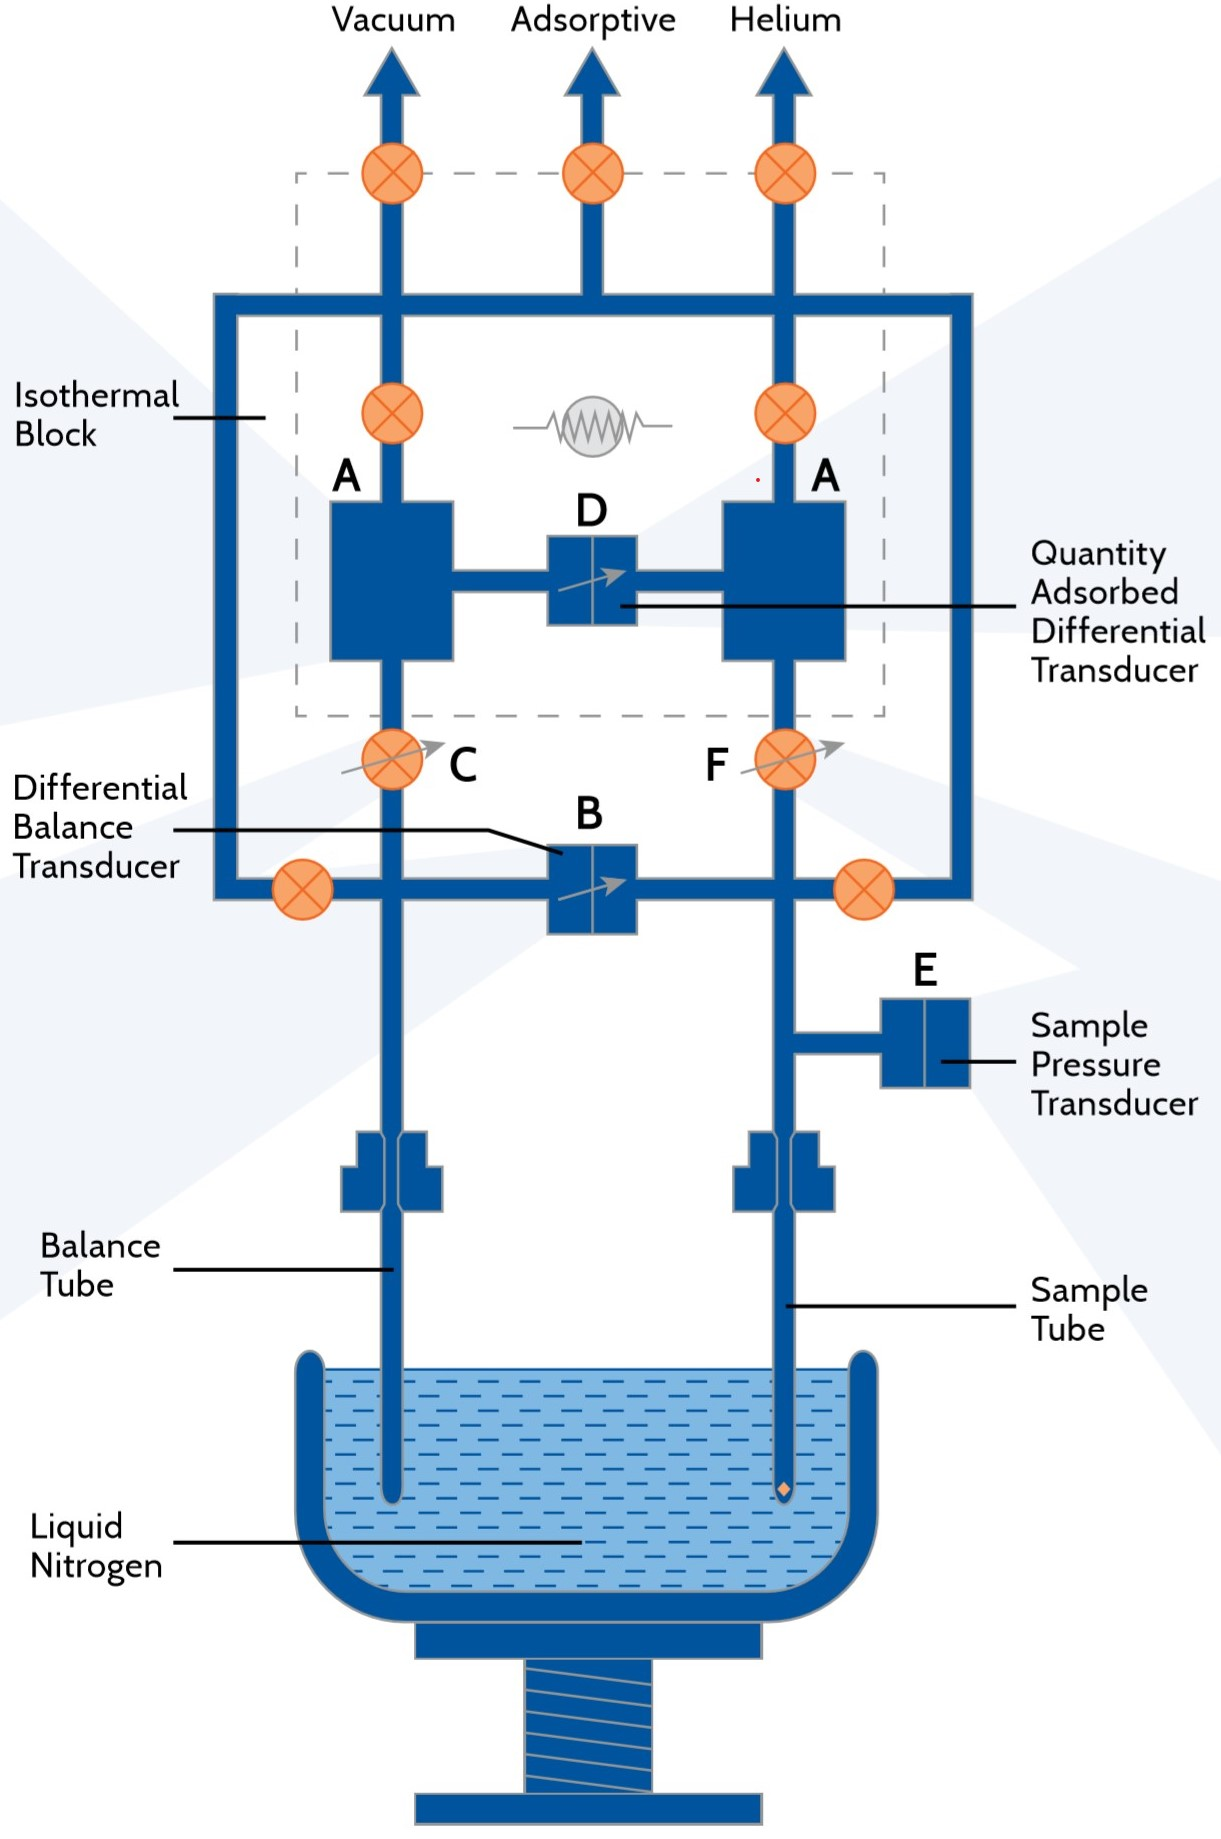
\includegraphics[width=0.6\textwidth]{Figures/ExperimentalSetup/Gemini-technique.jpg}
\medskip
\caption{The Gemini technique principle for surface area and pore volume determination \cite{gemini_brochure}}
\label{fig:gemini_technique}
\end{figure}

In order to remove any possible contaminants that could have absorbed onto the porous LIG structure, samples were degassed under a constant helium flux at ?XXX $\degree$C for ?X h before each measurement by using a dedicated unit. The values of the relative pressure varied from XXX to XX for the acquisition of the isotherm plot during the adsorption analysis. The empty volume of the test tube was determined helium gas injection measurement. 

The specific surface area $A_{BET}$ [$m^2/g$] was calculated for the relative pressure interval between XXX and XXX. The associated error was obtained by considering the microbalance uncertainty to be 0.01 $\mu g/cm^2$. Total Pore Volume (TPV) was calculated at a relative pressure of XXX for all the measurements, while BJH distributions were estimated on the adsorption isotherms.

\subsection{AFM Morphological Characterization of LIGs}

For the quantitative morphological and topological characterization of LIGs supported by different substrates the AFM investigation approach as described in the Section \ref{Borghi-theory} of the Theoretical part was chosen.

The round shaped, 10 mm in diameter, LIG samples were prepared on  various substrates as described in Table \ref{tab:borghi_afm_samples}. 

\begin{table}[H]
\centering
    \caption{The List of Samples Prepared for AFM analysis}
    \label{tab:borghi_afm_samples} 
\medskip
\medskip
\begin{tabular}{ l | l | l } 


	Sample $\#$ & LIG Type\footnotemark[1] & Substrate Material \\ [13px]\hline
	1  & LIGP & Kapton$^{TM}$ Film 50 $\mu$m \\ [13px]
	2  & LIGF & Kapton$^{TM}$ Film 50 $\mu$m \\ [13px]\hline
	3  & LIGP & Kapton$^{TM}$ Tape 50 $\mu$m//PDMS-8:1 \\ [13px]
	4  & LIGF & Kapton$^{TM}$ Tape 50 $\mu$m//PDMS-8:1 \\ [13px]


\end{tabular}
\end{table}
\footnotetext[1]{Laser settings as according to the Table \ref{tab:ligtypes}} 

The main interest was to investigate the morphological differences between the LIG ($i.e.$ LIGP and LIGF) supported by the the polyimide foil $in\:situ$ and the composite material LIG-PDMS.

The LIG samples were characterized by Atomic Force Microscopy (AFM) using a Multimode 8 microscope (Bruker) operated in Peak-Force Tapping Mode in air, equipped with silicon nitride cantilevers mounting single crystal silicon tips, with nominal radius 8-12 nm, resonance frequency in the range ??50-90 kHz??, and force constant ??k = 0.4 N/m??. Several 20 $\mu$m × 10 $\mu$m images were acquired with scan rate 0.5 Hz and sampling resolution 2048 × 512 points, in order to characterize the morphology of the interface. In order to remove artifacts due to sample tilt and scanner bow the images were flattened by line-by-line subtraction of first and second order polynomials. 


\section{Flexible Supercapacitors based on LIG}
The aim of this part of the project was to investigate the prospects of using LIG as an electrode material in thin and flexible symmetrical supercapacitor cells based on inorganic biocompatible electrolytes. It was assumed from the beginning that the LIG microstructure may have an impact on the electrochemical behaviour of the cells. Therefore various cell types based on LIGP and LIGF supported by three different flexible substrates, namely PI, PU and PDMS, were designed and prepared for the following investigations of their voltage behavior in charging/discharging experiments.

\subsection{LIG Based Electrodes. Design and Production}

A supercapacitor cell can be assembled in different ways. Main types include coin cells and Swagelok$^{TM}$ type cells. The latter is very popular in laboratory research as it can be cleaned and reused again for multiple times, whereas coin cells have to be dismantled after the experiments.  

\medskip
\textbf{Swagelok$^{TM}$ Setup}

First objective was to investigate the dependence of LIG electrostatic double-layer capacitance on its type and the substrate material in a series of cyclic voltammetry (CV) and Galvanostatic Cycling with Potential Limitation (GCPL) experiments incorporating the Swagelok$^{TM}$ cell type (see Figure \ref{fig:swagelok_cell}). The specifics of this setup is that the electrical contact between the collector and the electrode needs to be in the plane of the collector on the back side of the flat electrode. Therefore virtually no wiring can be used. Previously, a solution was found by LAMPSe group to solve a similar problem by integrating the Vertical Interconnect Access (VIA) \cite{dallinger_stretchable_2020}. Descriptive schematics are shown in Figure \ref{fig:Super_Cap_VIAS}. In a prepared round shaped $\varnothing 10\:mm$ LIG electrode a bunch of 24 small holes ($\varnothing \sim 80\:\mu m$, Figure \ref{fig:FM_VIAS_contact}) was laser-cut. For the PI it was found that depending on the laser settings and the hole diameter the edges around might remelt and close the hole just after laser impulse (Figure \ref{fig:PI_VIAS_contact}). Therefore the respective settings were found (Power 28$\%$ Speed 10$\%$ PPI 500 Z-defocus 1 mm ID5) which allowed to ensure that the cavities stayed open. These holes were small enough to not affect robustness and flexibility of the substrate materials. The cavities were then filled with silver ink (Leitsilber 200 from Ted Pella) and dried at 85 $\degree$C for 20 min. The porous structure of LIG as well as its satisfying wettability with silver ink allowed the liquid to spread into the electrode bulk, forming conductive thin LIG/Ag composite wires and providing a good electrical connection to the back side of the electrode. 

\begin{figure}[H]
\begin{subfigure}{0.33\textwidth}
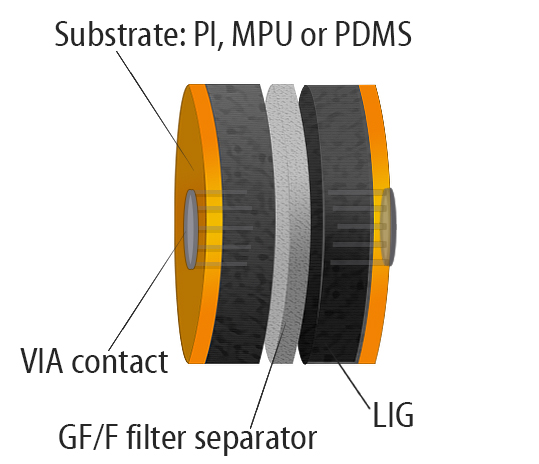
\includegraphics[width=0.95\textwidth]{Figures/ExperimentalSetup/Super_Cap_VIAS.jpg}
\captionsetup{width=0.9\linewidth}
\caption{LIG based supercapacitor with VIAs contacts}
\label{fig:Super_Cap_VIAS}
\end{subfigure}
\begin{subfigure}{0.33\textwidth}
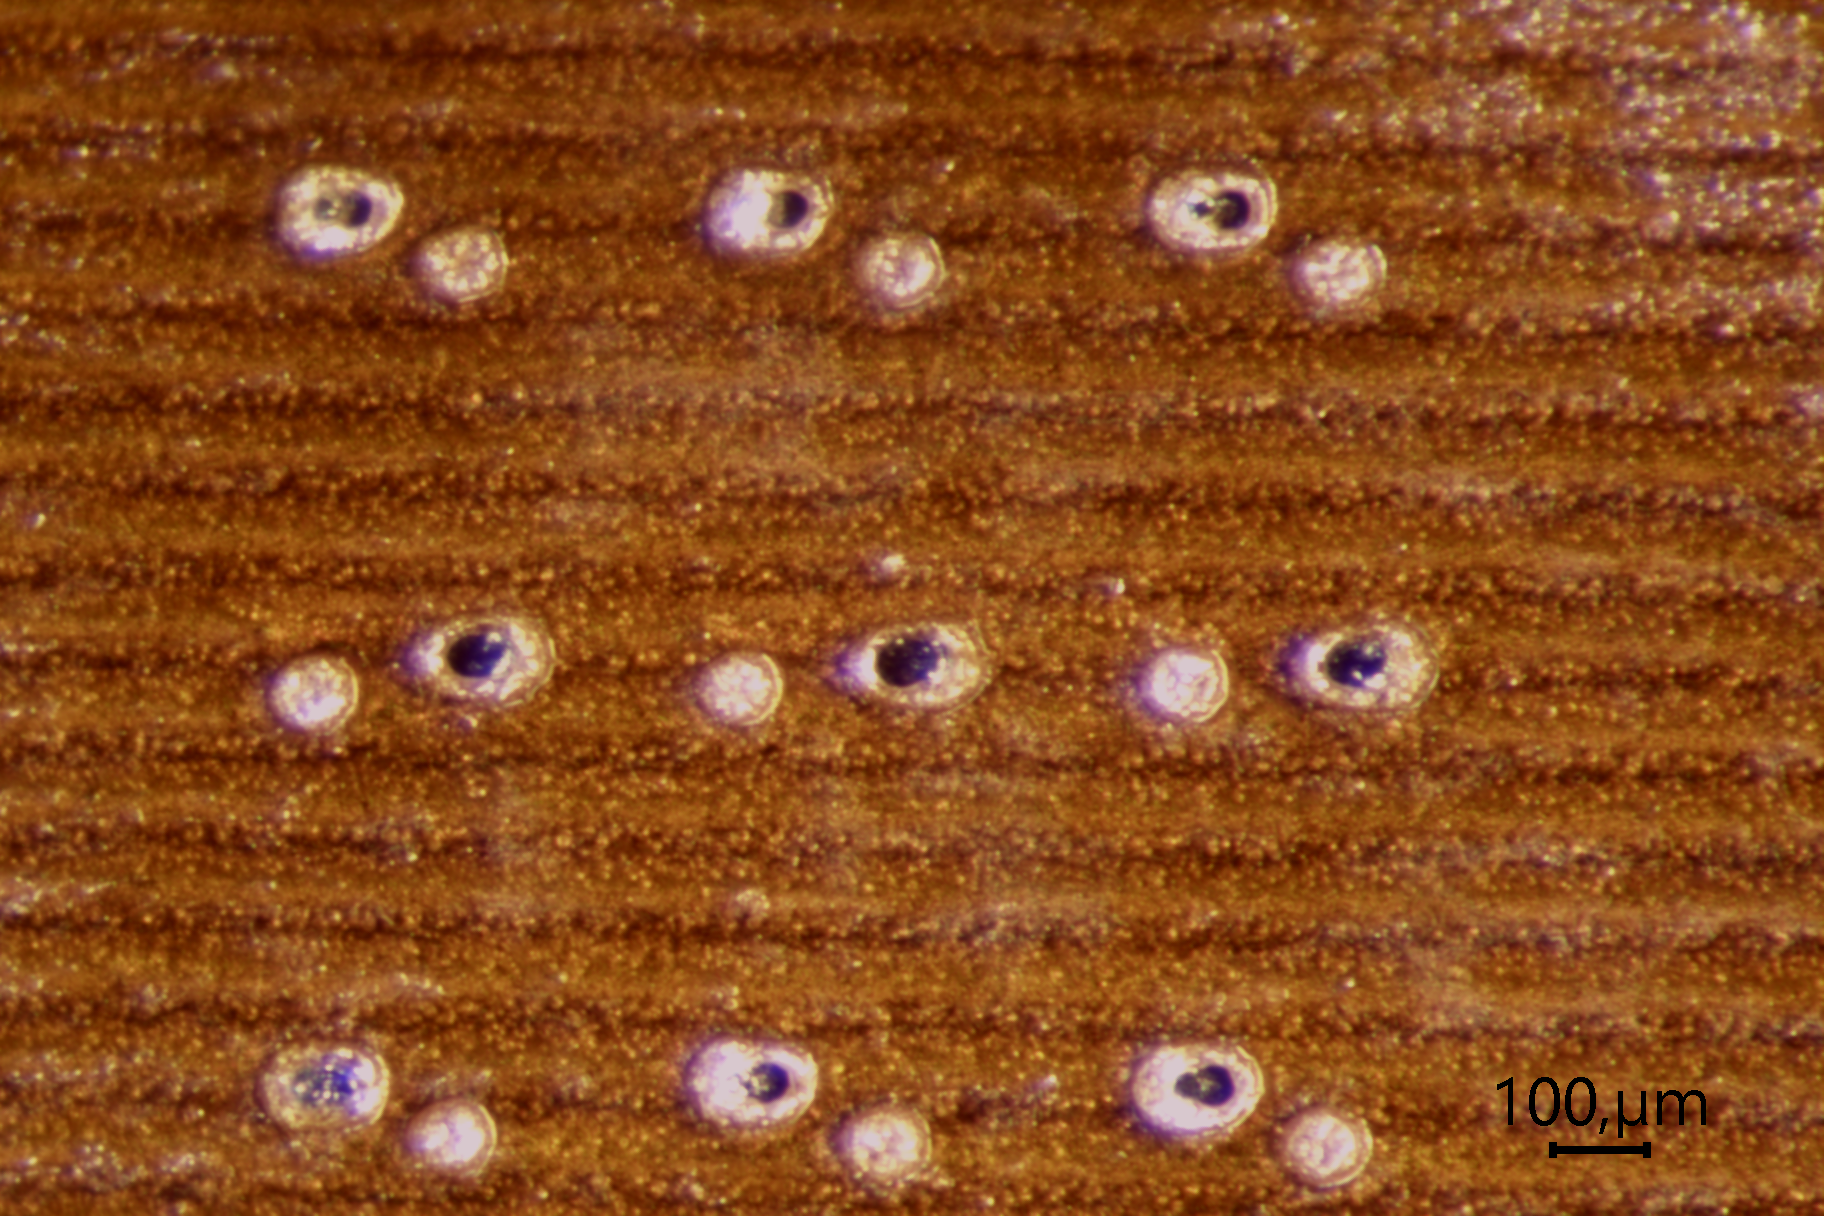
\includegraphics[width=0.95\textwidth]{Figures/ExperimentalSetup/Holes made after LIG strange white dots sample 13.png} 
\captionsetup{width=0.9\linewidth}
\caption{Partly closed laser-cut holes in PI}
\label{fig:PI_VIAS_contact}
\end{subfigure}
\begin{subfigure}{0.33\textwidth}
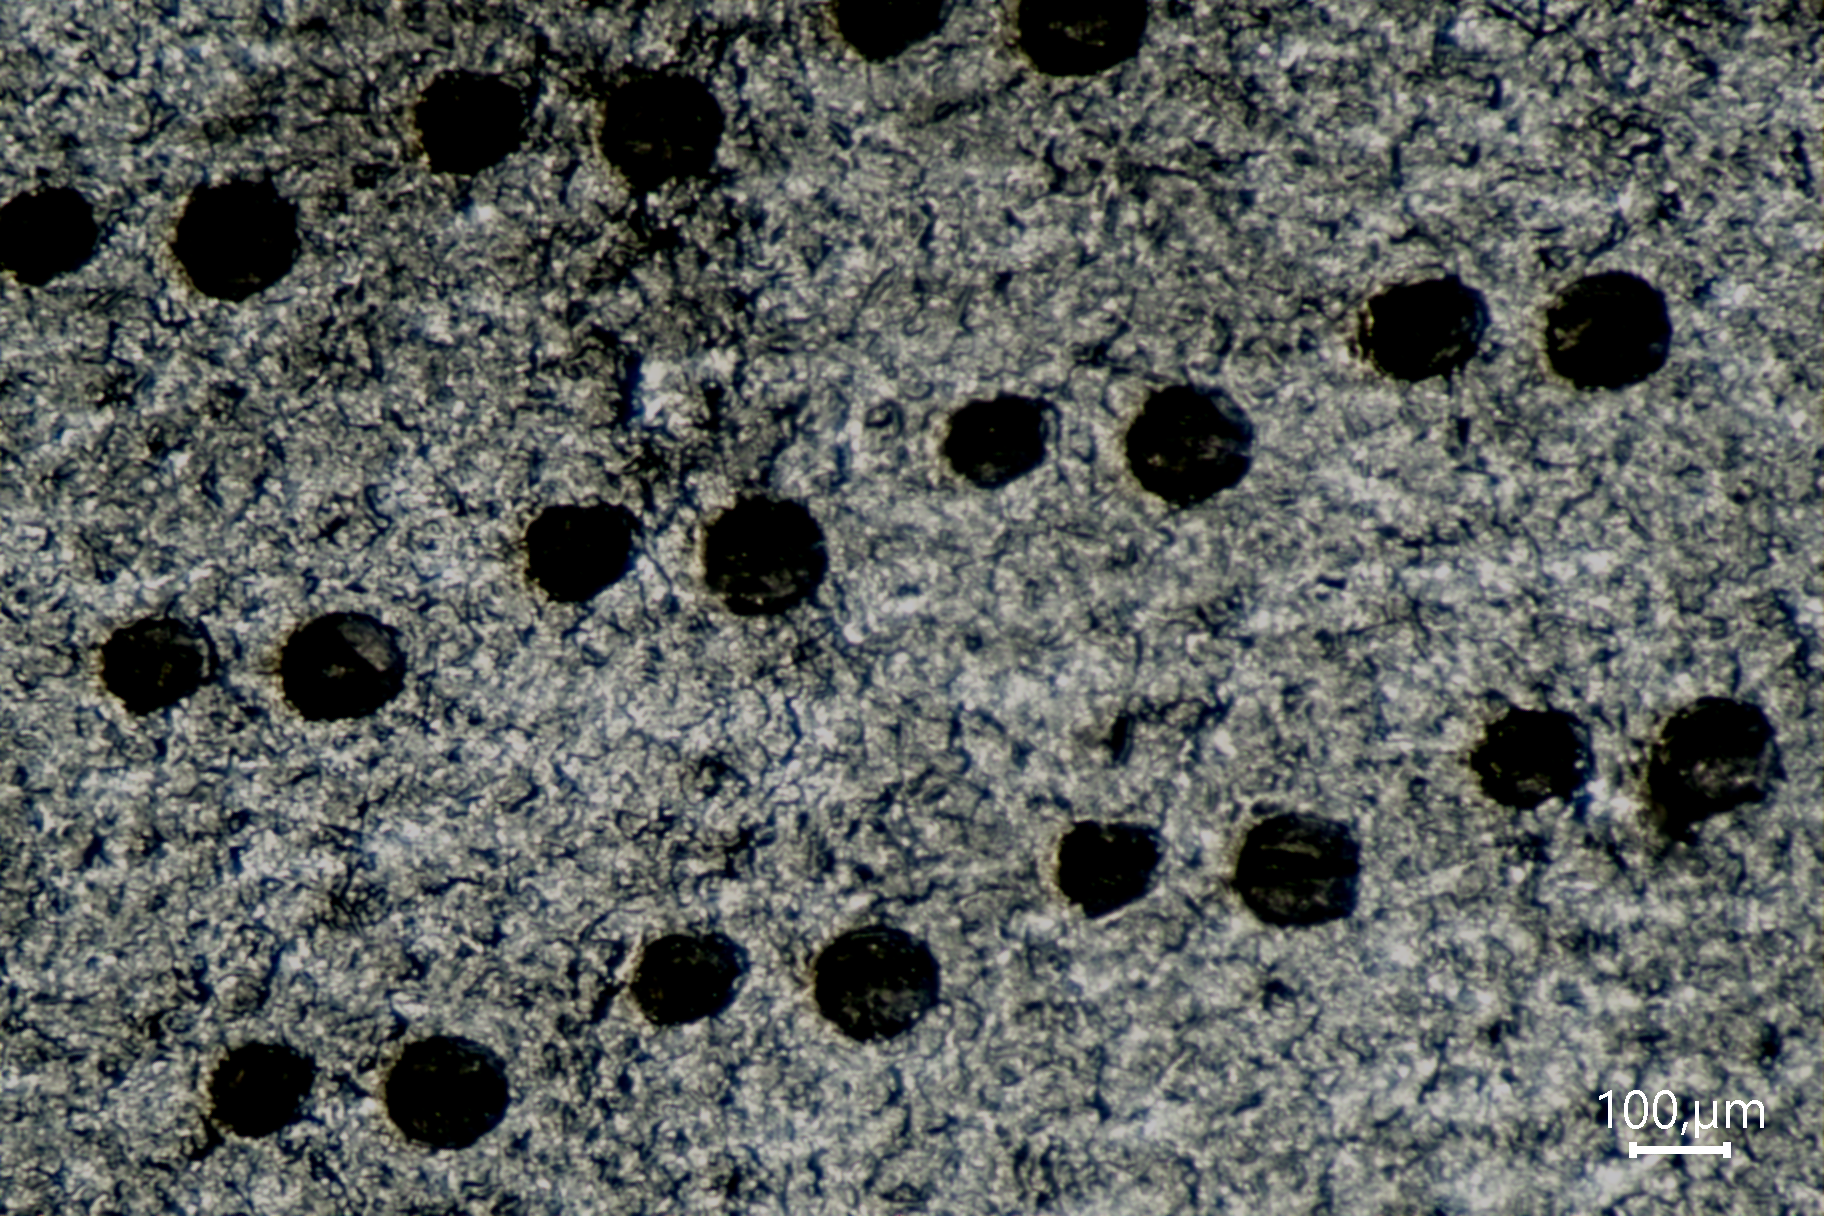
\includegraphics[width=0.95\textwidth]{Figures/ExperimentalSetup/FM VIAS contact holes.png}
\captionsetup{width=0.9\linewidth}
\caption{A set of see-through VIA holes in MPU}
\label{fig:FM_VIAS_contact}
\end{subfigure}
\medskip
\caption{Light microscope pictures of VIA contact holes and schematics of a LIG based supercapacitor}
\label{fig:VIAS_Supercapacitor}
\end{figure}

The electrical VIAS contacts of all prepared LIG electrodes was controlled before the Swagelok$^{TM}$ cells Type 2 were assembled as shown in Figure \ref{fig:swagelok_cell}. The Teflon$^{TM}$ housing contains two stainless steel collectors which enclose the investigated supercapacitor cell in the middle. Aqueous solution of sodium nitrate NaNO$_3$ (XXX name) in 1M concentration prepared from deionized $H_2O$ was used as an electrolyte. The glass microfibre filter (GF/F) had the thickness of XXX $\mu m$.
 
\begin{figure}[H]
\centering
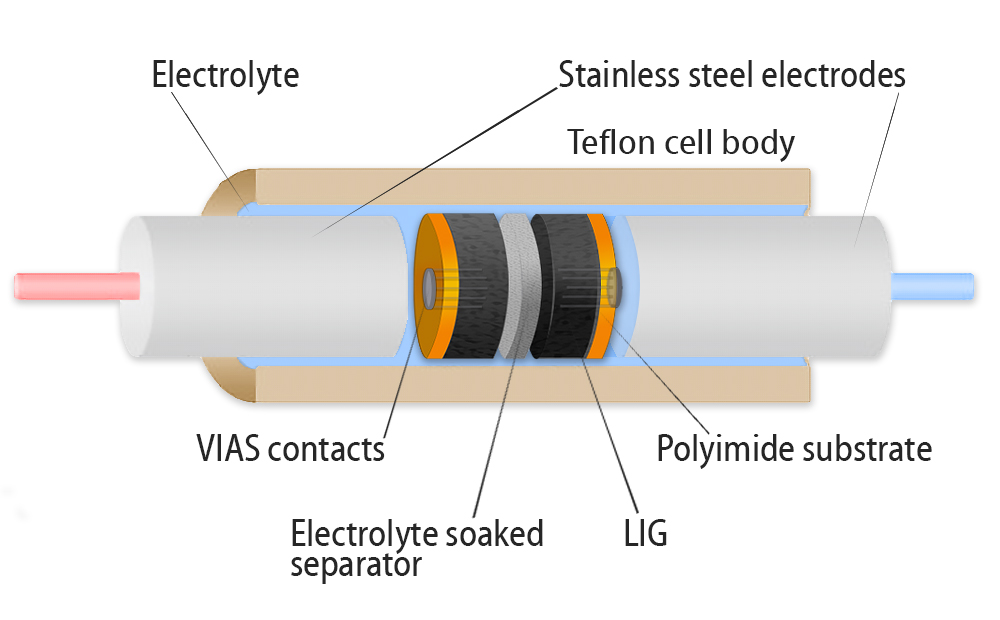
\includegraphics[width=0.8\textwidth]{Figures/ExperimentalSetup/Swagok_final.jpg}
\medskip
\caption{Swagelok$^{TM}$ cell setup for cyclic voltammetry experiments}
\label{fig:swagelok_cell}
\end{figure}


\textbf{Thin stretchable supercapacitor cells}

Encouraged by the preliminary results with Swagelok cells, which will be described in the Results Section \ref{chapter:Results and discussion}, the next step in this project was to demonstrate the feasibility of the LIG based flexible supercapacitors in conditions closer to industrial requirements. This required creating a bio friendly thin and stretchable supercapacitor cell, applicable for skin wearable devices. In that case the electrodes were prepared from LIG-PDMS-8:1 conductive composite in a form of a circle which had a 1.5 mm thin and 15 mm long protrusion. This protrusion "leg" had an advantage of being as flexible as the rest of the electrode and at the same time had the same conductivity as the rest which allowed it to be used as an electrical wiring contact as shown in Figure \ref{fig:LIG-PDMS-supercap}. 

\begin{figure}[H]
\centering

\includegraphics[width=0.6\textwidth]{Figures/Placeholder.jpg}
\medskip
\captionsetup{width=0.6\linewidth}
\caption{LIG-PDMS flexible thin supercapacitor device with composite wiring}
\label{fig:LIG-PDMS-supercap}
\end{figure}

Since the LIG has anisotropic resistivity the direction of laser treatment was chosen parallel to the "leg" axis in order to ensure the best electrical contact between the contact tip and the bulk of the LIG electrode. The two symmetrical LIG-PDMS-8:1 electrodes, separated by a XXX $\mu m$ thin GF/F separator, were then assembled in a cell. The MPU adhesive film was used as a sealing water impermeable housing. After assembly the interfacial volume of the cell was filled with 0.01 ml of 1M NaNO$_3$ or by 2M KOH (XXX) electrolyte solution prepared in deionized $H_2O$ by a syringe, the piercing hole was then closed by a small piece of MPU. The tips of the electrodes were terminated with commercially available Amphenol FCI Clincher Connectors (2 Position, Male) shown in Figure \ref{fig:SC_Amphenol_terminals}. 

\begin{figure}[H]
\centering
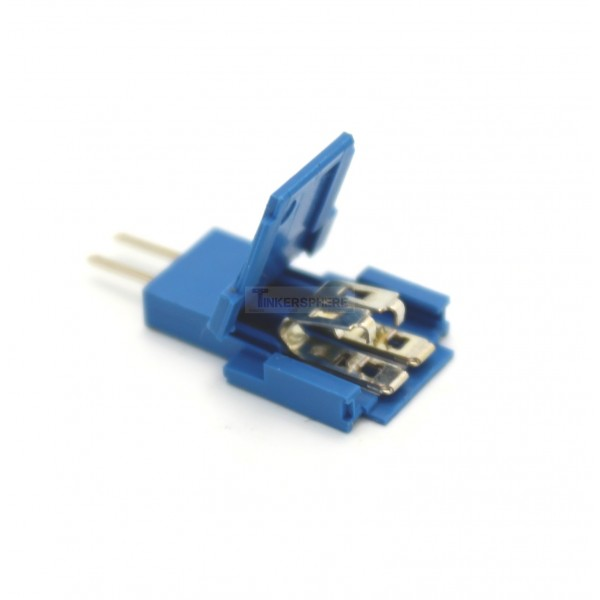
\includegraphics[width=0.3\textwidth]{Figures/ExperimentalSetup/amphenol-fci-clincher-connector-2-position-male.jpg}
\medskip
\caption{Amphenol FCI Clincher Connector \cite{Amphenol}}
\label{fig:SC_Amphenol_terminals}
\end{figure}



The Table \ref{tab:supercapacitor_electrodes} in the Results Section \ref{chapter:Results and discussion} indexes the details about all the  electrodes which were prepared and subsequently assembled into supercapacitor cells.

\subsection{Electrochemical Characterization}
Electrical performance of the assembled cells was investigated by the means of Cyclic Voltammetry (CV), Galvanostatic Cycling with  Potential Limitation (GCPL) as well as with Impedance Spectroscopy for a part of the cells. The measurements were performed with potentiostat MPG-2 Device operated by EC-Lab$^{TM}$ software at Institute of Chemistry and Technology of Materials at TU Graz.

 The CV method involves linearly varying, $i.e$ sweeping, an electrode potential between two limits at a specific scanning rate while recording the current that flows through the electrochemical cell. After the voltage reaches a certain maximum value, the potential is reversed and so is the current as well. The test involves a certain amount of cycles repeated one after another. The variation of the voltage in time can be seen in \ref{fig:CV-1}. The change in the potential causes a respective current response, which in case of the two-electrode setup is recorded as the function the voltage difference between the two leads connected to the cell as shown in Figure \ref{fig:CV-2}. The graph contains information about the electrochemical response of the system, which can be chemical reactions happening during the measurement as the potential changes or/and charge storage. For the supercapacitors the final curve shape helps to evaluate which of the two known charge storage mechanisms (electric double layer (EDL) or the faradaic charge transfer) is involved into the operation of the device. For the EDL cells, in which no redox reactions taking place, the ideal cycle has a rectangular shape, as this corresponds to the situation of a maximum charge storage in absence of a non-linear $I(V)$ behaviour. Undesired chemical reactions on electrode can be avoided kinetically by choosing high enough scanning rates, or thermodynamically by selecting the right potential window where the materials stay chemically inactive. The latter is preferable for the materials with high inner resistance as the higher scanning rates may hinder the diffusion of the charges to the micro- and mesopores of the electrodes, which is necessary for the storage to happen.
 
 
\begin{figure}[H]
\begin{subfigure}{1\textwidth}
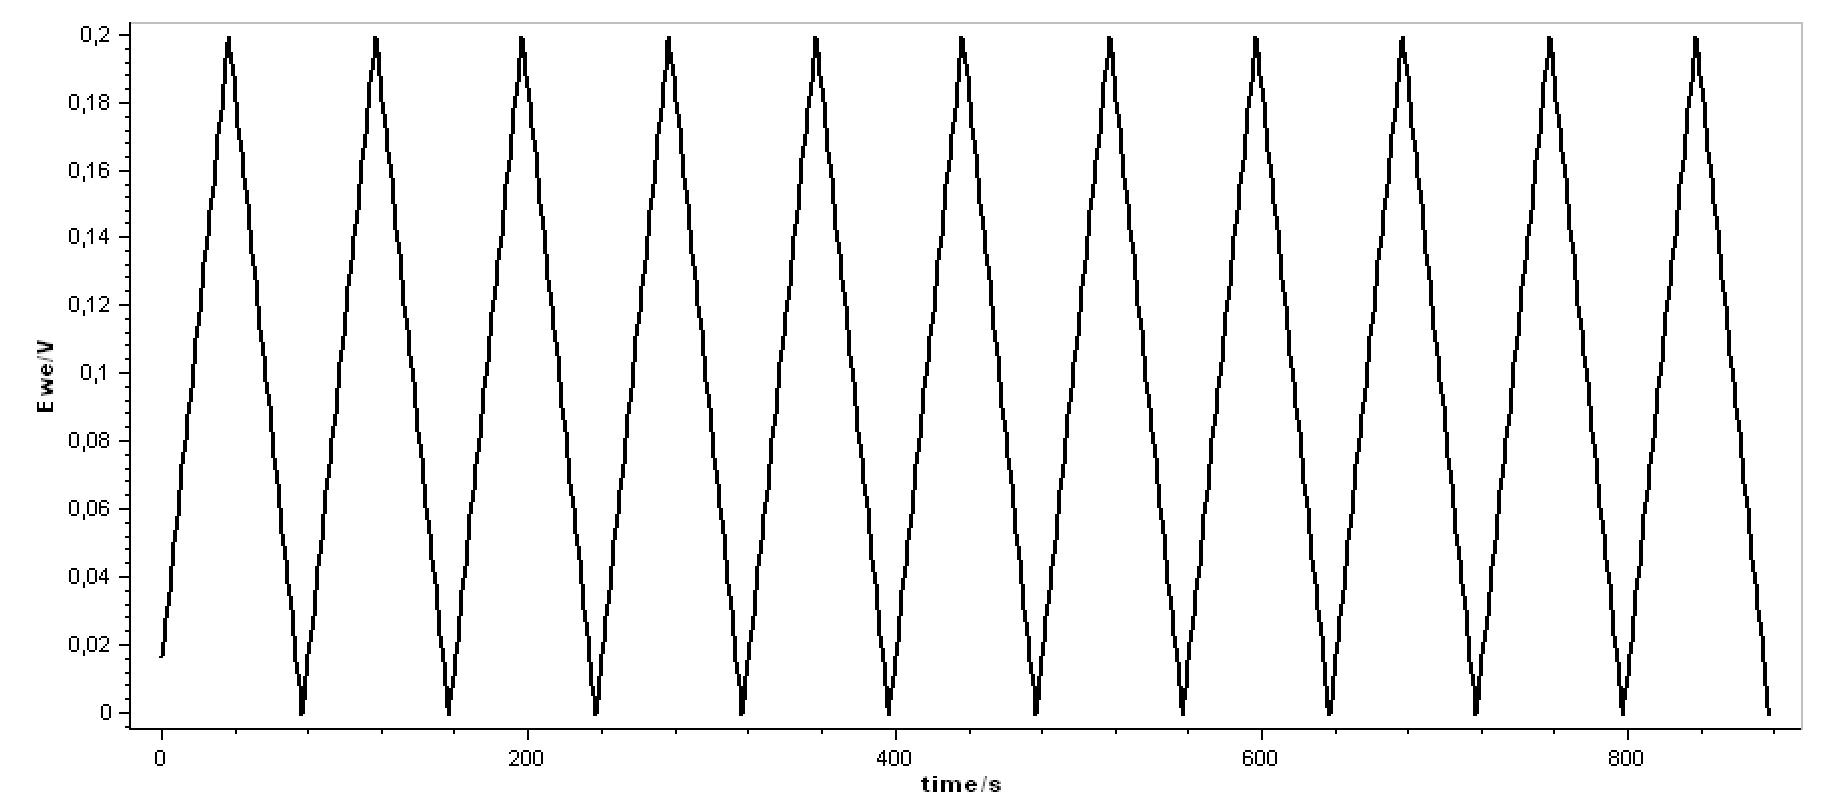
\includegraphics[width=0.95\textwidth]{Figures/ExperimentalSetup/CV-Voltage-time.jpg}
\captionsetup{width=0.9\linewidth}
\caption{Takes from EC-Lab$^{TM}$ potential versus time program for CV showing the forward and reversed linear potential ramp}
\label{fig:CV-1}
\end{subfigure}
\begin{subfigure}{1\textwidth}
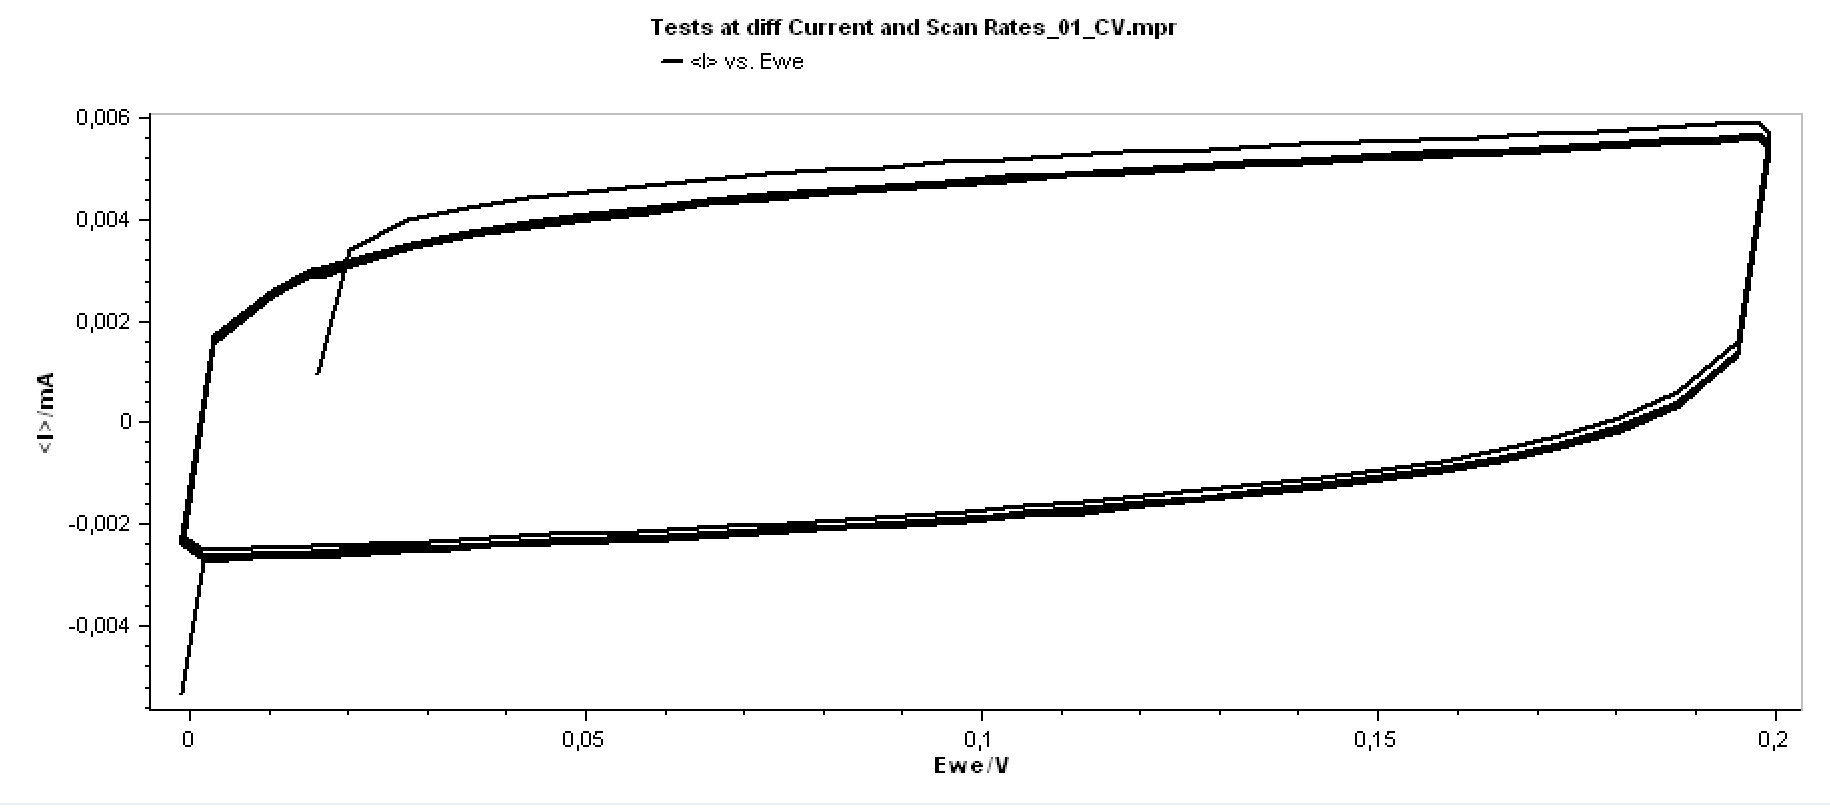
\includegraphics[width=0.95\textwidth]{Figures/ExperimentalSetup/CV-Voltage-I.jpg} 
\captionsetup{width=0.9\linewidth}
\caption{Cyclic Voltammogram of measured current versus applied potential}
\label{fig:CV-2}
\end{subfigure}
\medskip
\caption{Experimental data recorded during a CV test}
\label{fig:CV}
\end{figure}

 
 Together with the CV measurements the method of Galvanostatic Cycling with  Potential Limitation (GCPL) was employed. In these tests one cycle consists of the two stages. At first the device is charged at a constant current until the pre-defined potential difference between the two electrodes is achieved. After that the cell is discharged with the opposite current down to the zero potential. The method is widely utilized in supercapacitor characterization as not only it allows to estimate the principal electrical characteristics of the cells but also their cycling stability and performance over time. Similar to CV, the characteristic shapes of $V(t)$ GCPL curves (shown in Figure \ref{fig:GCPL-typical}) and their deviations allow to make estimations regarding the storage mechanisms taking place in the device. EDL cells with low inner resistance have triangular appearance and no potential drop at the beginning of the discharging stage. Potential scanning $dE/dt$ rates which are defined as the slope of the charging and discharging branches of the graph, together with the chosen value of the applied current have a great impact on the shapes of the curves and therefore have to be accurately selected.
 
 In order for the electrical properties evaluated by cyclic voltammetry to be comparable to the data obtained in galvanostatic experiments, the measurements with each cell were performed in series and as good as it was achievable for the common voltage potential ranges. 
 
 \begin{figure}[H]
\centering
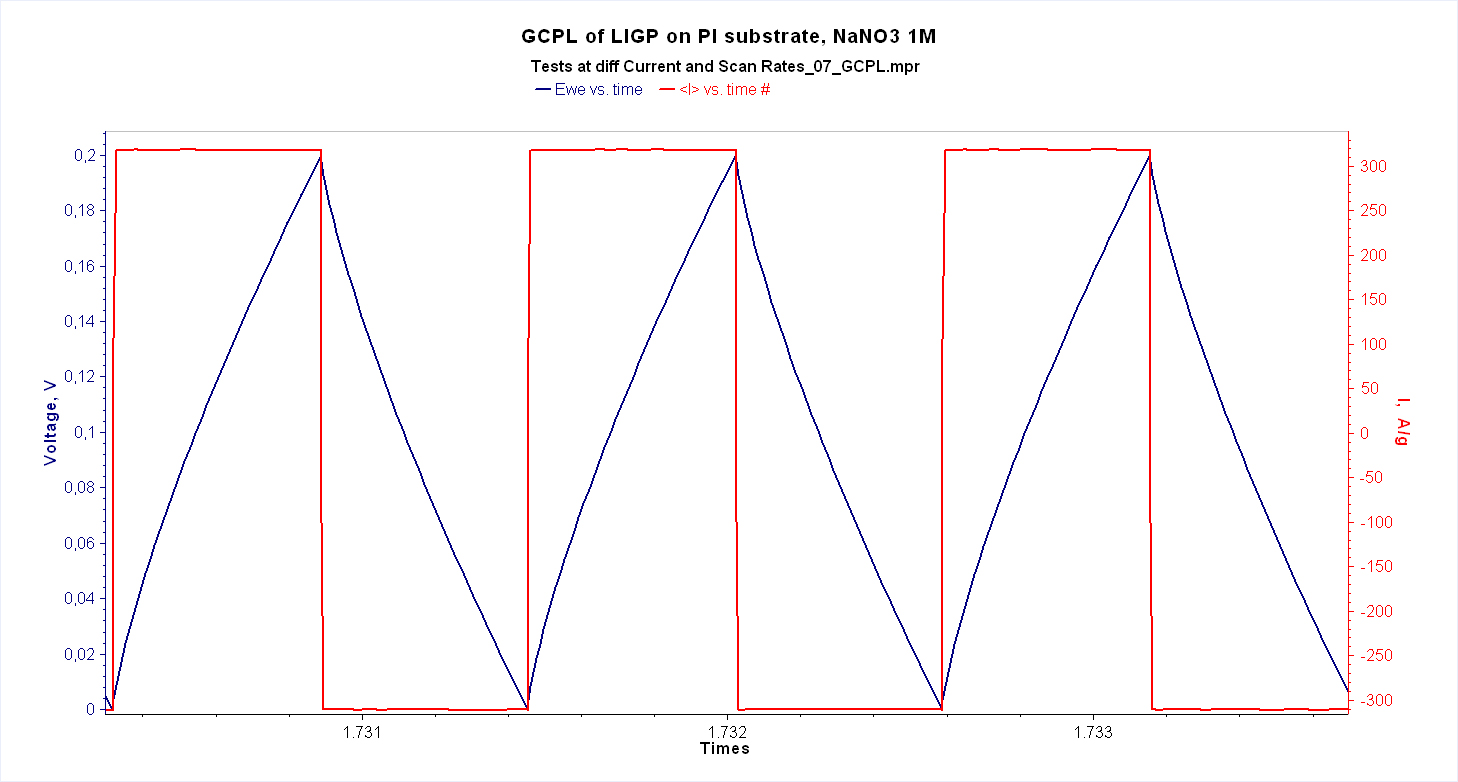
\includegraphics[width=0.9\textwidth]{Figures/ExperimentalSetup/Galvanostatic-charge_discharge_cell_1_I_V_time.jpg}
\medskip
\caption{Experimental data recorded during Galvanostatic charge-discharge cycling with potential limitation}
\label{fig:GCPL-typical}
\end{figure}

Each device was cycled at ambient temperature ($\sim19\degree$C). The settings of the measurements for the Swagelok cells can be found in Table \ref{tab:Electrochemistry-settings-Sw}.

\begin{table}[H]
\centering
    \caption{CV and GCPL experiment settings for Swagelok Cells}
    \label{tab:Electrochemistry-settings-Sw} 
\medskip
\medskip
\begin{tabular}{l|l|l||l|l}
\hline
  &
\multicolumn{2}{c||}{Cyclic Voltammetry} &
\multicolumn{2}{c}{GCPL} \\
\hline
\pbox{100px}{.\\Electrode\\Type} & Sweeps [V] & $dV/dt$ [mV/s] & $V_{max}$ [V] & $I$ [mA] \\[13px]
\hline
\multirow{4}{*}{LIG-PI} & 0 - 0.2 & 5/10/20/50/100/200 & 0.2 & 0.04 - 1 \\[13px]
   &0 - 0.2/0.3/0.4/0.5 & 5 & 0.2 - 0.5 & 0.1 \\[13px]
   &0 - 0.6/0.7/0.8/0.9/1.0/1.1/1.2 & 5 & 0.6 - 1.2 & 0.1 \\[13px]
\hline
\multirow{4}{*}{LIG-PDMS} & 0 - 0.2 & 5/10/20/50/100/200 & 0.2 & 0.08 - 1.6 \\[13px]
    &0 - 0.2/0.3/0.4/0.5 & 5 & 0.2 - 0.5 & 0.2 \\[13px]
\hline
\multirow{5}{*}{LIG-MPU} & 0 - 0.1 & 2 & 0.1 & 0.018 \\[13px]
    &0.1 - 0.2 & 2 & 0.2 & 0.018 \\[13px]
    &0 - 0.3 & 2 & 0.3 & 0.018 \\[13px]
    &0 - 0.4 & 2 & 0.4 & 0.018 \\[13px]
    & 0 - 0.2\footnotemark[1] & 5/10/20/50/100/200 & - & -\\[13px]
\hline

\end{tabular}
\end{table}

\footnotetext[1]{This device could not be identified as the type of LIG was not put in the protocol. However the CV curves showed very good behaviour}


The next series of CV and GCPL experiments was performed with the thin cells, the respective settings are presented in Table \ref{tab:Electrochemistry-settings-Thin}.

The retrieved data allowed to calculate relevant for the supercapacitor devices electrical characteristics. Capacitance of a cell was calculated from the CV curves by employing Equation \ref{eq:Capacitance-CV}:

\begin{equation}
\label{eq:Capacitance-CV}
C_{(CV)} = \frac{1}{2\times (dV/dt)_{CV} \times(V_2-V_1)}\times \oint_{V_1}^{V_2} I(V) dV
\end{equation}

and from the GCPL data with Equation \ref{eq:Capacitance-GC}:

\begin{equation}
\label{eq:Capacitance-GC}
C_{(GCPL)} = \frac{I_{discharge}}{(dV/dt)_{GCPL}}
\end{equation}

Where $(dV/dt)_{CV}\:[V/s]$ is the CV scan rate; $V_2,\: V_1\: [V]$ - the limits of the CV potential sweep; $I(V)\:[A]$ - CV current curve; $I_{discharge}$ - GCPL current at discharge; $(dV/dt)_{GCPL}$ - slope of the discharge part of a GCPL curve.


Specific gravimetric capacitance $C_g\:[F/g]$ and specific areal capacitance $C_A\:[\mu F/cm^2]$ were calculated with Equations \ref{eq:C-g} and \ref{eq:C-A} respectively:

\begin{equation}
\label{eq:C-g}
C_g = \frac{C}{m}
\end{equation}

\begin{equation}
\label{eq:C-A}
C_A = \frac{C}{s}
\end{equation}

Where $m\:[g]$ is the total mass of an active material on both electrodes; $s\:[cm^2]$ - total area of the active positive and negative electrodes.

Specific energy gravimetric and areal densities - $E_g\:[Wh/g]$ and $E_A\:[\mu Wh/cm^2]$:

\begin{equation}
\label{eq:E-g}
E_g = \frac{1}{2} \times C_g \times \frac{\Delta V^2}{3600}
\end{equation}

\begin{equation}
\label{eq:E-A}
E_A = \frac{1}{2} \times C_A \times \frac{\Delta V^2}{3600}
\end{equation}

With the knowledge about $\Delta t\:[s]$ discharge time in a respective GCPL experiment specific gravimetric and areal power densities, $P_g\:[W/g]$ and $P_A\:[\mu mW/cm^2]$, were calculated as follows:

\begin{equation}
\label{eq:P-g}
P_g = \frac{E_g}{\Delta t} \times 3600
\end{equation}

\begin{equation}
\label{eq:P-A}
P_A = \frac{E_A}{\Delta t} \times 3600
\end{equation}

Equations \ref{eq:Capacitance-GC} - \ref{eq:P-A} were adapted from Peng $et\: al.$ \cite{peng_flexible_2015}.


\textbf{Impedance Spectroscopy}

XXX IN PROCESS








